\documentclass[12pt]{article}
\usepackage[margin=1in]{geometry}
\usepackage{amsmath, amssymb, amsthm, graphicx, hyperref}
\usepackage{enumerate}
\usepackage{fancyhdr}
\usepackage{multirow, multicol}
\usepackage{tikz}
\pagestyle{fancy}
\fancyhead[RO]{Sicong Liu}
\fancyhead[LO]{MA-UY 2314: Discrete Mathematics}
\usepackage{comment}
\newif\ifshow
\showfalse
\begin{document}

\begin{center}
\textbf{\Large Homework 5}\\
\end{center}
\hrule

\vspace{0.2cm}
\begin{enumerate}
\item None
\item
\noindent 14.6 
\textbf{\begin{enumerate}[(a).]
\item $R=\{(x,y):|x-y| \leq 2\}$
\item R is reflexive. Assume $a \in A,$,NTS $(a,a) \in R$\\
$a-a=0 \leq 2 \to (a,a) \in R$
\item R is not irreflexive. Assume $a \in A,$,NTS $(a,a) \in R$\\
$a-a=0 \leq 2 \to (a,a) \in R$
\item R is symmetric. Assume $(a,b) \in R$, NTS $(b,a) \in R$\\
$\to |a-b| \leq 2$\\
$\to |b-a| \leq 2$\\
$\to (b,a) \in R$
\item R is not antisymmetric. Counterexample:
$(1,2) \in R, (2,1) \in R, 1 \neq 2$
\item R is not transitive. Counterexample:
$(1,3) \in R, (3,5) \in R, (1,5) \notin R$
\end{enumerate}}

14.7(d) $R^{-1}=\{(x,y):x,y \in \mathbf{N}, y|x\}$\\
Prove: let $E=\{(x,y):x,y \in \mathbf{N}, y|x\}$\\
NTS (1) $(x,y) \in R^{-1} \longrightarrow  (x,y) \in E$\\
(2) $(x,y) \in E \longrightarrow (x,y) \in R^{-1}$\\
Prove of (1): Assume $(x,y) \in R^{-1} \longrightarrow (y,x) \in R$\\
$\longrightarrow y|x$\\
$\longrightarrow (x,y) \in E$\\
Prove of (2): Assume $(x,y) \in E \longrightarrow y|x$\\
$\longrightarrow (y,x) \in R$\\
$\longrightarrow (x,y) \in R^{-1}$\\

14.7(e)  $R^{-1}=\{(x,y):x,y \in \mathbf{Z}, yx > 0\}$\\
Prove: let $E=\{(x,y):x,y \in \mathbf{Z}, yx > 0\}$\\
NTS (1) $(x,y) \in R^{-1} \longrightarrow  (x,y) \in E$\\
(2) $(x,y) \in E \longrightarrow (x,y) \in R^{-1}$\\
Prove of (1): Assume $(x,y) \in R^{-1} \longrightarrow (y,x) \in R$\\
$\longrightarrow yx > 0$\\
$\longrightarrow (x,y) \in E$\\
Prove of (2): Assume $(x,y) \in E \longrightarrow yx > 0$\\
$\longrightarrow (y,x) \in R$\\
$\longrightarrow (x,y) \in R^{-1}$\\

\item 14.12 $R=(\{(x,y):x,y \in \mathbf{Z}, x \leq y\}$\\
$R^{-1}= \{(x,y):x,y \in \mathbf{Z}, y \leq x\}$\\
Prove: let $E=\{(x,y):x,y \in \mathbf{Z}, y \leq x\}$\\
NTS (1) $(x,y) \in R^{-1} \longrightarrow  (x,y) \in E$\\
(2) $(x,y) \in E \longrightarrow (x,y) \in R^{-1}$\\
Prove of (1): Assume $(x,y) \in R^{-1} \longrightarrow (y,x) \in R$\\
$\longrightarrow y \leq x$
$\longrightarrow (x,y) \in E$\\
Prove of (2): Assume $(x,y) \in E \longrightarrow y \leq x$\\
$\longrightarrow (y,x) \in R$\\
$\longrightarrow (x,y) \in R^{-1}$\\

\item 14.13(a) $A=\{1,2\},R=\{(1,1)\}$\\
14.13(b) $A=\emptyset, R=\emptyset$

\item 14.14 Prove: $R  \; is \; symmetric \Longleftrightarrow R=R^{-1}$\\
NTS (1) $R \;  is \; symmetric \longrightarrow R=R^{-1}$\\
(2) $R=R^{-1} \longrightarrow R \;  is \; symmetric$\\
Prove of (1):\\
NTS (a) $R \subseteq R^{-1}$\\
(b) $R^{-1} \subseteq R$\\
Prove of (a): let $(x,y) \in R \longrightarrow (y,x) \in R \longrightarrow (x,y) \in R^{-1}$\\
Prove of (b): let $(x,y) \in R^{-1} \longrightarrow (y,x) \in R \longrightarrow (x,y) \in R$\\
\vspace{0.05in}
Prove of (2): let $(x,y) \in R \longrightarrow (y,x) \in R^{-1} \longrightarrow (y,x) \in R \longrightarrow R \;  is \; symmetric$\\

14.15 Prove: $R  \; is \; antisymmetric \Longleftrightarrow R \cap R^{-1} \subseteq \{(a,a):a \in A\}$\\
NTS (1) $R  \; is \; antisymmetric \longrightarrow R \cap R^{-1} \subseteq \{(a,a):a \in A\}$\\
(2)  $R \cap R^{-1} \subseteq \{(a,a):a \in A\} \longrightarrow R  \; is \; antisymmetric$\\
Prove of (1): let $(x,y) \in R \longrightarrow (y,x) \in R \longrightarrow x=y$\\
$(y,x) \in R^{-1} \longrightarrow (x,y) \in R^{-1} \longrightarrow (x,y) \in R \cap R^{-1} \wedge (x,y) \in \{(a,a):a \in A\} \longrightarrow R \cap R^{-1} \subseteq \{(a,a):a \in A\}$\\
Prove of (2): let x R y $\wedge$ y R x $\longrightarrow$ x R y $\wedge$ x $R^{-1$} y $\longrightarrow (x,y) \in R \cap R^{-1}$\\
$(x,y) \in \{(a,a):a \in A\} \longrightarrow x=y \longrightarrow R  \; is \; antisymmetric$\\

\item 14.17
\[
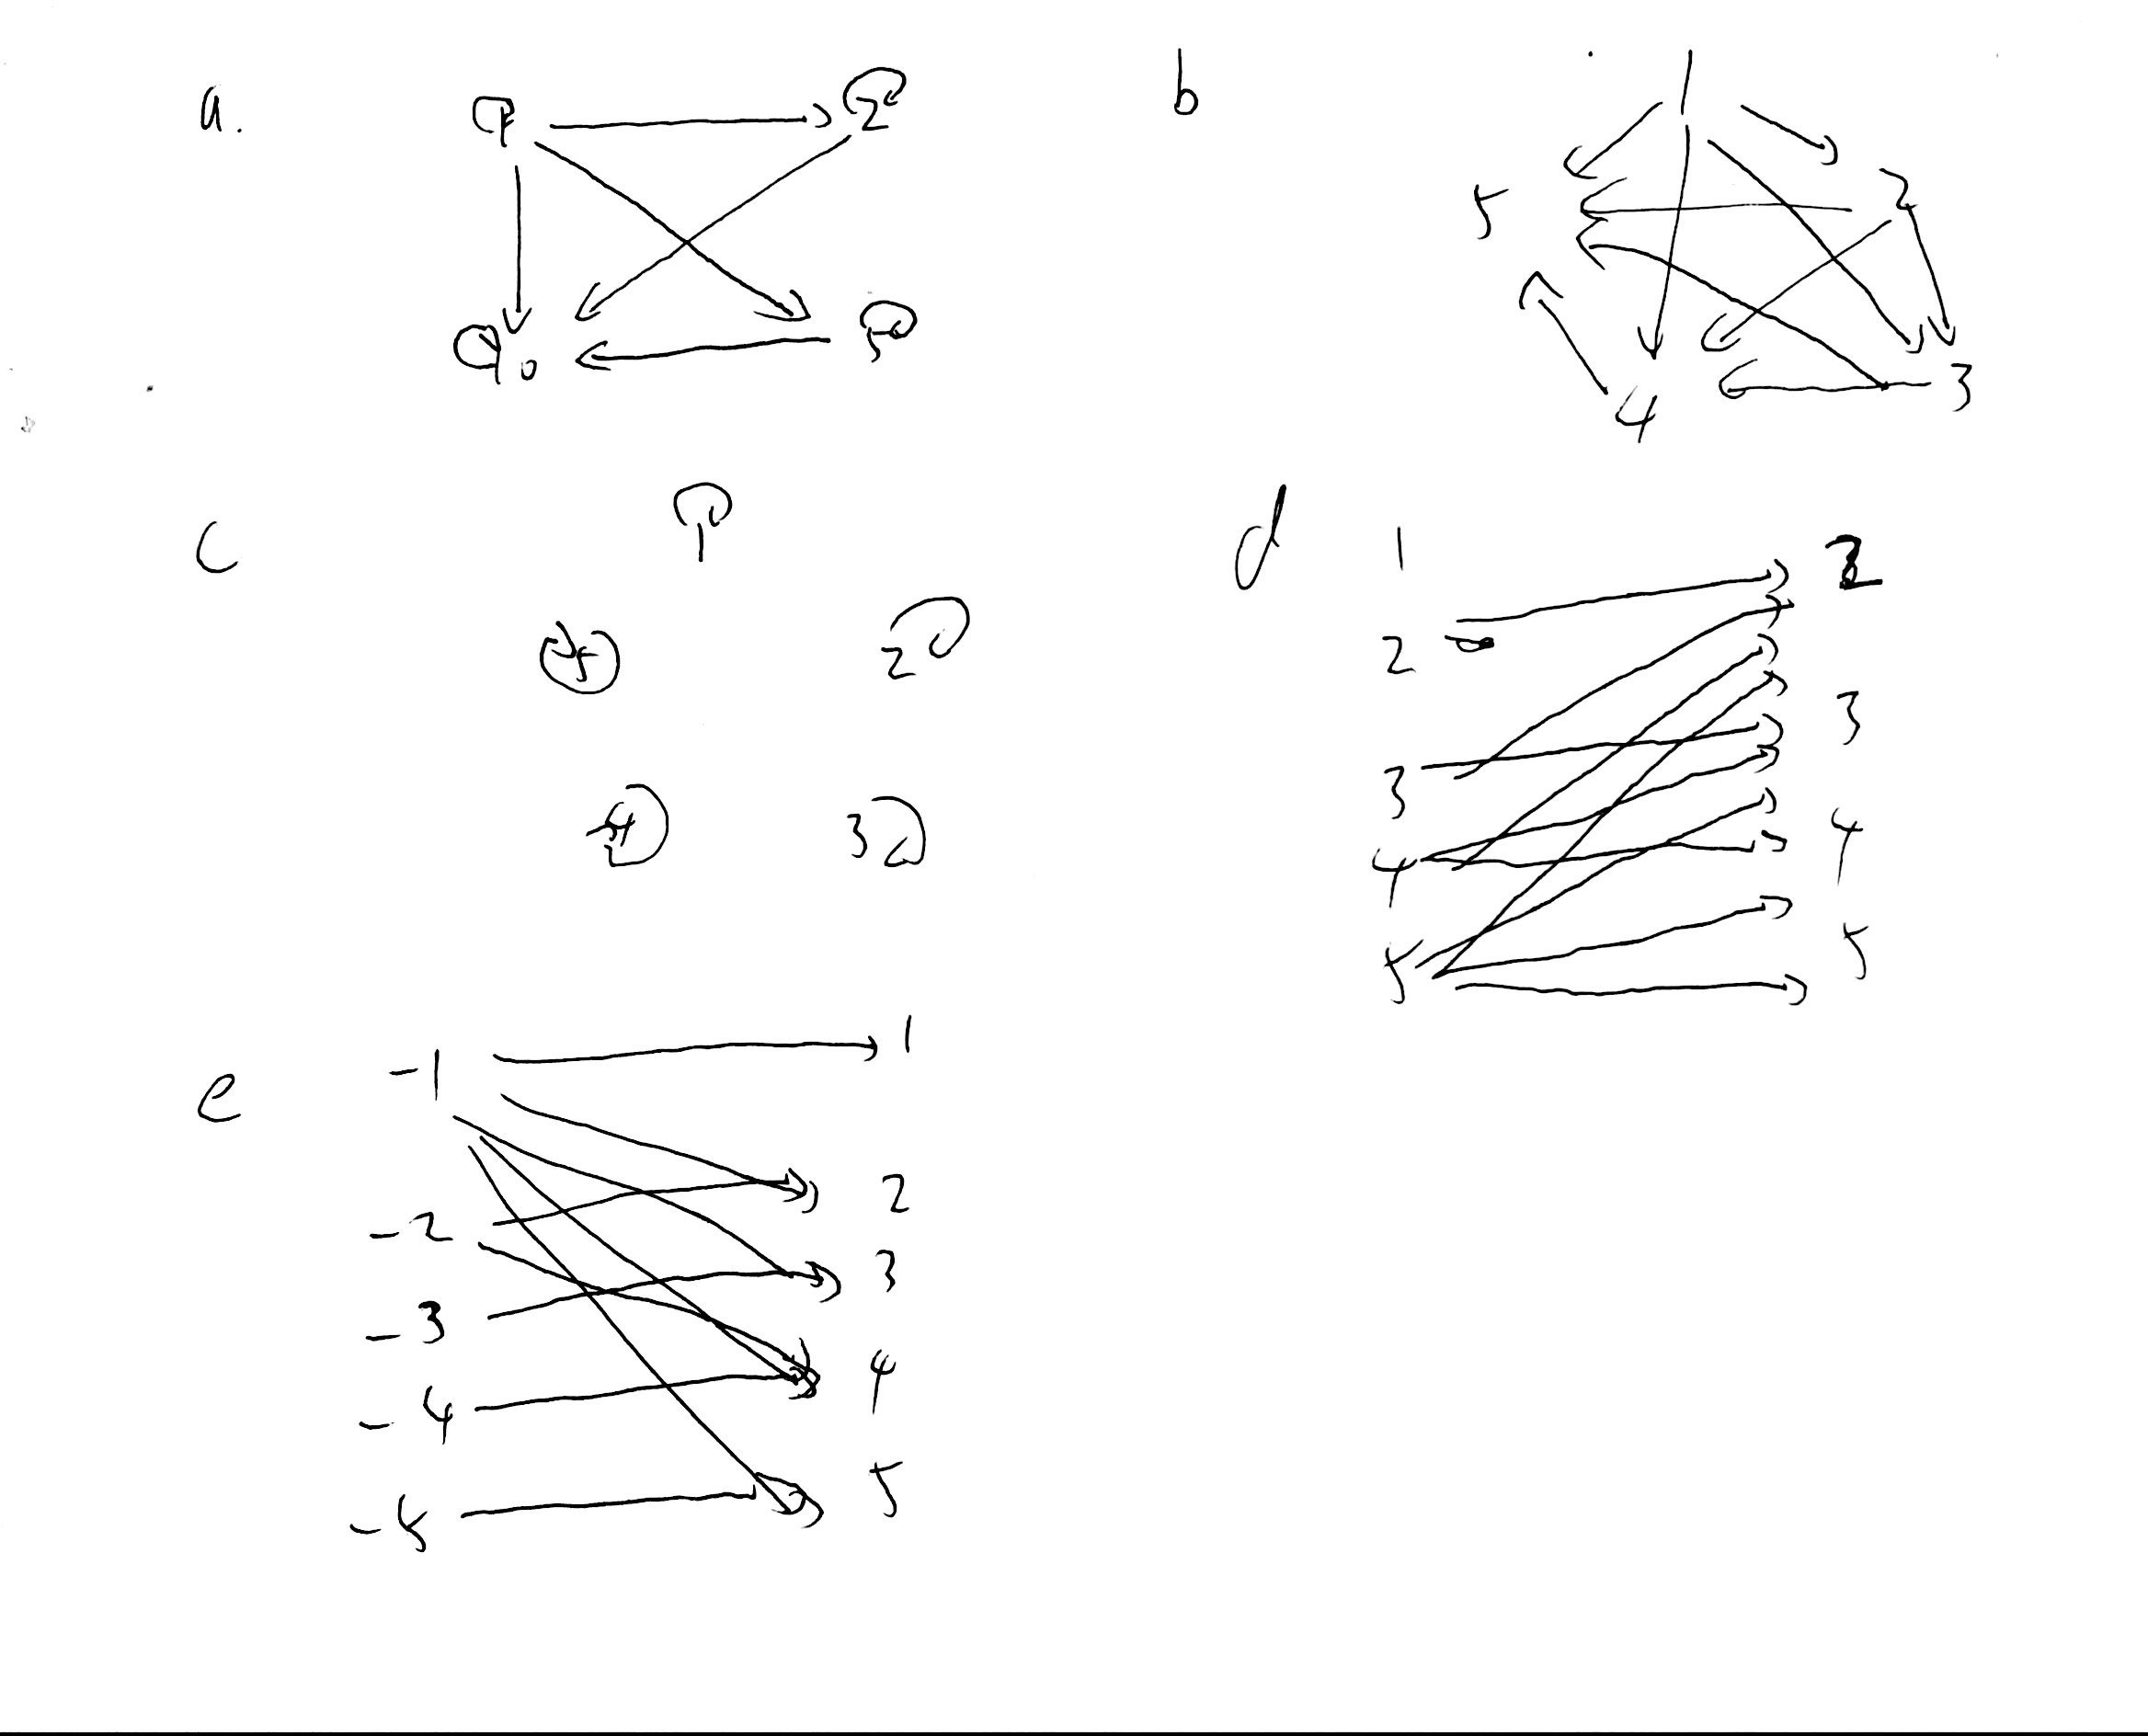
\includegraphics[width = 5in, height = 4in]{image.JPG} %your jpg file goes between the curly brackets.  To size it, play around with the syntax between the square brackets.  
\]
\end{enumerate}
\end{document}